\textbf{\textit{(5) Let $\cT=\{\sigma_1,\dots,\sigma_m\}$ be a triangulation of a full-dimensional point configuration $\cA=(\aaa_1,\dots,\aaa_n)\subset\RR^d$ of $n$~points, where we consider the $\sigma_i\in\binom{[n]}{d+1}$ to be index sets. Let $R^{\text{int}}$ be the set of interior ridges, defined to be intersections $\rho = \rho_{ij} = \sigma_i\cap\sigma_j$ of two facets of~$\cT$ such that the affine span of the points of~$\cA$ indexed by~$\rho$ has dimension~$d-1$. (In the triangulations of~Figure~\ref{fig:triangs1}, they are the interior edges.)}}

  \begin{figure}[htbp]
    \centering
    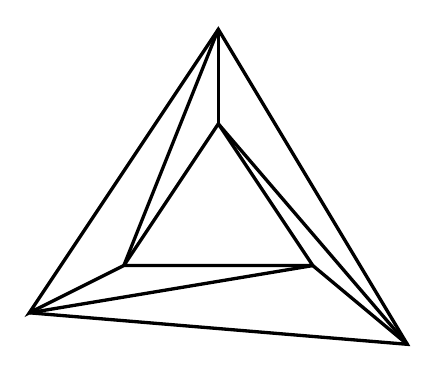
\begin{tikzpicture}[scale=.4]
      \coordinate (1) at (0,0);
      \coordinate (2) at (12,-1);
      \coordinate (3) at (6,9);
      \coordinate (4) at (3,1.5);
      \coordinate (5) at (9,1.5);
      \coordinate (6) at (6,6);

      \draw[very thick] (1)--(2)--(3)--(1)--(4)--(5)--(6)--(4);
      \draw[very thick] (2)--(5);
      \draw[very thick] (3)--(6);

      \draw[very thick] (1)--(5);
      \draw[very thick] (2)--(6);
      \draw[very thick] (3)--(4);
    \end{tikzpicture}
    \qquad
    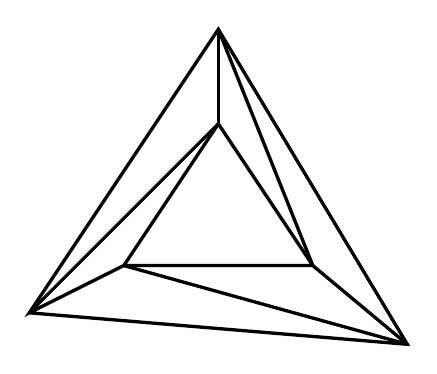
\begin{tikzpicture}[scale=.4]
      \coordinate (1) at (0,0);
      \coordinate (2) at (12,-1);
      \coordinate (3) at (6,9);
      \coordinate (4) at (3,1.5);
      \coordinate (5) at (9,1.5);
      \coordinate (6) at (6,6);

      \draw[very thick] (1)--(2)--(3)--(1)--(4)--(5)--(6)--(4);
      \draw[very thick] (2)--(5);
      \draw[very thick] (3)--(6);

      \draw[very thick] (2)--(4);
      \draw[very thick] (3)--(5);
      \draw[very thick] (1)--(6);
    \end{tikzpicture}    
    \caption{Two triangulations.
    View the source code for the coordinates of the points.}
    \label{fig:triangs1}
  \end{figure}

\begin{enumerate}
  \item
      \textbf{\textit{For a vector $\omega\in\RR^n$, lift the points in $\cA$ to heights~$\omega$, so that $\cA^\omega=\big(\binom{\aaa_1}{\omega_1},\dots,\binom{\aaa_n}{\omega_n}\big)$. For each interior ridge $\rho=\sigma_i\cap\sigma_j\in R^{\text{int}}$, formulate the folding condition that expresses that $\rho$ indexes a face of the lower convex hull of~$\cA^\omega$, in terms of the coordinates of the~$\aaa_i$ and~$\omega$. Your folding condition should be an inequality that is linear in each height~$\omega_i$.}}

To formulate the folding condition, we make use of Definition 7.4 in Rheka R. Thomas~\footnote{Rekha R. Thomas. Lectures in geometric combinatorics., volume 33 of Student Mathematical Library. Providence, RI: American Mathematical Society (AMS); Princeton, NJ: Institute for Advanced Studies, 2006.}:
        \begin{equation*}
            \begin{split}
                \rho \text{ indexes a face of the lower convex hull of } \cA^\omega & \Leftrightarrow \rho \text{ indexes a folded face of the regular subdivision } \\
                & \Leftrightarrow \exists \pmb{y} \in \mathbb{R}^{d} \text{ s.t. } \left\lbrace \begin{array}{l} (\pmb{y}, -1) \cdot (\pmb{a_j}, \omega_j)^t = 0 \forall j \in \rho \\ (\pmb{y}, -1) \cdot (\pmb{a_j}, \omega_j)^t < 0 \forall j \not\in \rho \end{array} \right.
            \end{split}
        \end{equation*}
    geometrically, this means that $(\pmb{y}, -1)$ is normal to the face $\rho$ is indexing (in the lifted configuration) and all other points lie \textit{above} it.
    Note that, in contrast to the example in Rheka Thomas, $\rho$ does not index a face of the regular subdivision since it's affine span has dimension $d-1$. 
    In this case, the face in the lifted configuration \textit{folds} to a ridge in the original point configuration.

  \item
        \textbf{\textit{Write code that takes the coordinates of the $\aaa_i$ and the facets $\sigma_i$ of a triangulation as input, and outputs the set of folding conditions in a text file in LP file format.}}

  \item
    Download a linear programming software such as
    \texttt{gurobi},
    \texttt{cplex} or
    \texttt{scip}/\texttt{soplex}
    and check explicitly whether there exists a choice of heights $\omega$ that induces each of the triangulations of Figure~\ref{fig:triangs1}.

  \item
    Using this code,
    check that the triangulation of the $4$-dimensional cube 
    given by the files \texttt{4-cube.vertices} and \texttt{4-cube.triangulation}
    is non-regular, i.e., it does not come from a lifting to~$\RR^5$.
    If you like, download and play with TOPCOM.
  \end{enumerate}
